\documentclass[parskip=half]{scrbook}

\title{Title}
\subtitle{Subtitle}
\author{Firstname Lastname}
\date{1 January 2020}

\def\titlethesistype{Master Thesis}
\def\titlesupervisor{Supervisor Name}

\usepackage[utf8]{inputenc}

% Math
\usepackage{amsmath}
\usepackage{amsthm}
\newtheorem{definition}{Definition}[section]
\newtheorem{theorem}{Theorem}
\usepackage{amssymb}
\let\emptyset\varnothing

% SI Units
\usepackage[binary-units]{siunitx}
\sisetup{detect-all}

% References
\usepackage[numbers]{natbib}
\bibliographystyle{plainnat}

% Color
\usepackage{xcolor}
\definecolor{linkcolor}{cmyk}{1.0, 0.6, 0.0, 0.56}

% Links
\usepackage{hyperref}
\hypersetup{
	colorlinks = true,
	citecolor  = linkcolor,
	linkcolor  = linkcolor,
	urlcolor   = linkcolor,
}
\urlstyle{same}
\usepackage[noabbrev]{cleveref}
\crefname{lstlisting}{listing}{listings}
\Crefname{lstlisting}{Listing}{Listings}

% Tables
\usepackage{booktabs}
\usepackage{tabularx}

% Graphics
\usepackage{tikz}
\usetikzlibrary{arrows.meta}
\usetikzlibrary{calc}
\usetikzlibrary{positioning}
\usepackage{graphicx}
\usepackage{wrapfig}

% Code
\usepackage{listings}
\lstset{
	basicstyle=\ttfamily\footnotesize,
	breaklines=true,
	breakatwhitespace=false,
	showstringspaces=false,
	numbers=left,
	tabsize=4,
	numberbychapter=false,
	captionpos=b,
	frame=leftline,
	framesep=2mm,
	xleftmargin=8mm
}
\usepackage[outputdir=out]{minted}
\usemintedstyle{tango}
\setminted{
	fontsize=\footnotesize,
	tabsize=4,
	linenos,
	frame=leftline,
	framesep=2mm,
	xleftmargin=10mm
}
% The 'listings' environemnt is defined by minted, yet uses a different counter.
\AtBeginEnvironment{listing}{\setcounter{listing}{\value{lstlisting}}}
\AtEndEnvironment{listing}{\stepcounter{lstlisting}}
% Fix listoflistings command.
\providecommand{\listoflistings}{\lstlistoflistings}

% Title
\usepackage{titlepage}

% Page
\usepackage{appendix}
\usepackage[margin=2.5cm,bottom=3cm,footskip=1cm]{geometry}
\usepackage{showframe}
\usepackage{chngcntr}
\setcounter{tocdepth}{2}
\setcounter{secnumdepth}{2}
\counterwithout{equation}{chapter}
\counterwithout{figure}{chapter}
\counterwithout{table}{chapter}

% Font
\usepackage{microtype}
\usepackage{newtxtext,newtxmath}
\usepackage[scale=0.88]{sourcecodepro}
\usepackage[T1]{fontenc}

% Custom packages
\usepackage{lipsum}

\begin{document}

\frontmatter
\maketitle
\tableofcontents
\listoffigures
\listoftables
\listoflistings

\chapter*{Abstract}

Abstract paragraph.

\mainmatter

\chapter{Running Text}

\section{Lorem Ipsum}

\lipsum[1-2]

\section{Modifiers}

The most important text modifiers are \emph{emphasis} and \texttt{teletype}.

\section{References}

This section explains various ways of include references.
Use footnotes for less important references.

\subsection{Hyperlinks}

Official university website: \url{https://www.uibk.ac.at/}

\subsection{Footnotes}

This text has a footnote\footnote{Footnote content goes here.} attached to it.

\subsection{Citations}

The book \emph{Principles of Program Analysis}~\cite{Nielson:ppa} is referenced here.

\subsection{Blockquotes}

Some text before a blockquote.

\begin{quote}
	\lipsum[3]
\end{quote}

Some text after a blockquote.

\section{Lists}

\subsection{Bullets}

\begin{itemize}
	\item One entry in the list
	\item Another entry in the list
	      \begin{itemize}
		      \item Nested list element
	      \end{itemize}
\end{itemize}

\subsection{Enumeration}

\begin{enumerate}
	\item One entry in the list
	\item Another entry in the list
	      \begin{enumerate}
		      \item Nested list element
	      \end{enumerate}
\end{enumerate}

\subsection{Description}

\begin{description}
	\item[First] One entry in the list
	\item[Second] Another entry in the list
\end{description}

Alternatively you may force line breaks after the descriptor.

\begin{description}
	\item[First]\hfill\\
	      One entry in the list
	\item[Second]\hfill\\
	      Another entry in the list
\end{description}

\section{Math}

\subsection{Inline Math and Display Math}

These are your basic math environments.
Inline math is recommended for short, concise expression, like $n = 42$ or $\mathcal{R} = \emptyset$.
Display math should be used for more complex stuff:

$$f(x) = \int_{-\infty}^\infty \hat f(\xi)\,e^{2 \pi i \xi x} \,d\xi$$

\subsection{Equations with Numbers}

This text refers to \cref{eq:some_equation}.

\begin{equation}\label{eq:some_equation}
	x^2 + y^2 = z^2
\end{equation}

\subsection{Theorem Environments}

\begin{definition}
	We simply define $x = 13$.
\end{definition}

\begin{theorem}
	Let's say $x$ is equal to $13$.
\end{theorem}

\begin{proof}
	Proof by definition.
\end{proof}

\subsection{Units}

Leverage the \texttt{siunitx} package to properly typeset numbers and units.
\num{12345678} and \SI{9.81}{\meter\per\second^2}.

\chapter{Other Elements}

This section shows you how to add other elements, like figurs or tables, to your document.

\section{Tables}

\subsection{Simple}

\begin{center}
\begin{tabular}{lrr}
	\toprule
	Description & Count & Price (single)\\
	\midrule
	Soda & 6 & 2.49 €\\
	Coffee & 2 & 3.19 €\\
	Sandwich & 1 & 5.39 €\\
	\bottomrule
\end{tabular}
\end{center}

\subsection{Specific Width}

\begin{center}
\begin{tabularx}{0.75\textwidth}{Xrr}
	\toprule
	Description & Count & Price (single)\\
	\midrule
	Soda & 6 & 2.49 €\\
	Coffee & 2 & 3.19 €\\
	Sandwich & 1 & 5.39 €\\
	\bottomrule
\end{tabularx}
\end{center}

\subsection{With Caption}

\Cref{tbl:some_table} as a caption and can be referenced.
Note that by using the \texttt{table} environment, the table is no longer inline and is repositioned automatically.

\begin{table}
	\centering
	\begin{tabularx}{0.75\textwidth}{Xrr}
		\toprule
		Description & Count & Price (single)\\
		\midrule
		Soda & 6 & 2.49 €\\
		Coffee & 2 & 3.19 €\\
		Sandwich & 1 & 5.39 €\\
		\bottomrule
	\end{tabularx}
	\caption{This table has a caption.}
	\label{tbl:some_table}
\end{table}

\section{Graphics}

Avoid having inline figures.
Always give them a caption and reference them in text.

\subsection{Figures}

See \cref{fig:some_figure}.

\begin{figure}
	\centering
	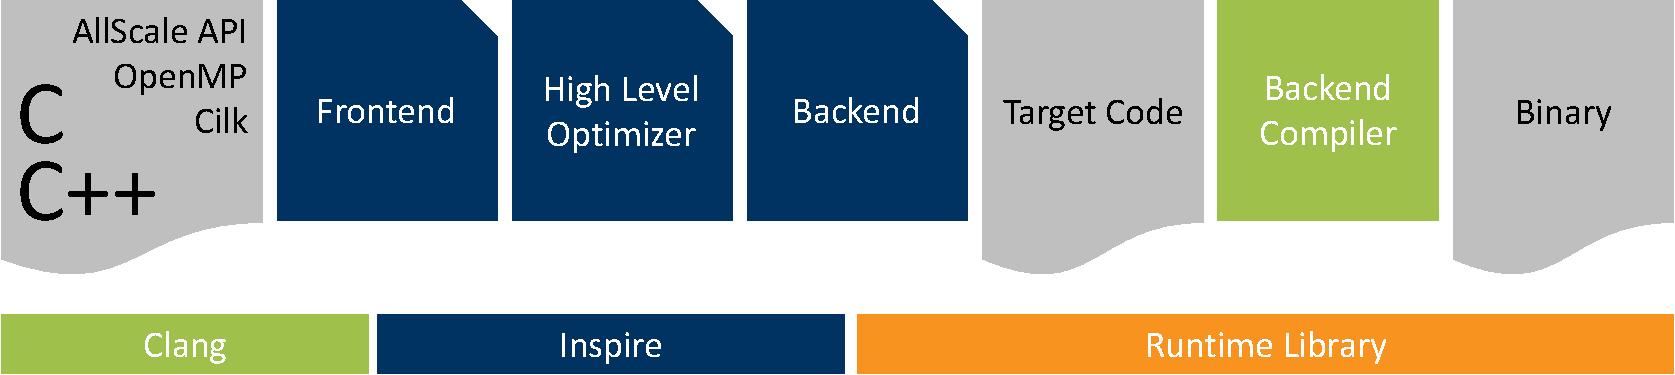
\includegraphics[width=0.9\textwidth]{images/example.pdf}
	\caption{An example image.}
	\label{fig:some_figure}
\end{figure}

\subsection{TikZ}

See \cref{fig:tikz_figure}.

\begin{figure}
	\centering
	% 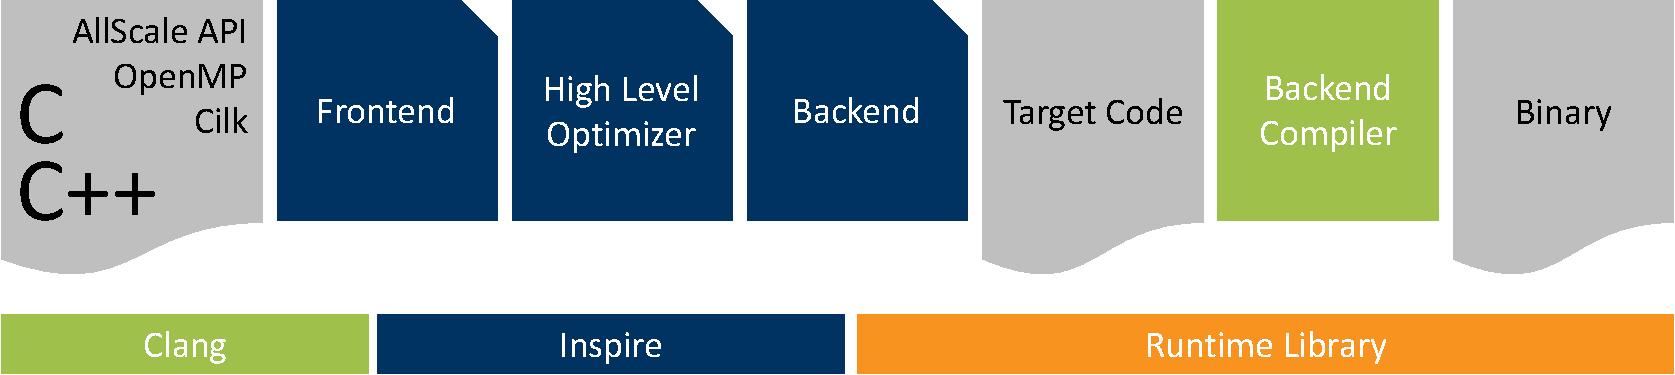
\includegraphics[width=0.9\textwidth]{images/example.pdf}
	%\usetikzlibrary{arrows.meta}
%\usetikzlibrary{positioning}

\tikzstyle{ptr} = [
	-{Latex[length=1.8mm]},
	dashed,
	shorten <= 0.2cm,
	shorten >= 0.2cm,
	bend left
]

\begin{tikzpicture}[every node/.style={minimum width=1cm},
                    level 1/.style={sibling distance=4.5cm},
                    level 2/.style={sibling distance=2.0cm}]

	\node (1) {\{\}}
		child {
			node (2) {$=$}
			child { node (3) {$a$} }
			child { node (4) {$6$} }
		}
		child {
			node (5) {$=$}
			child { node (6) {$b$} }
			child { node (7) {$7$} }
		}
		child {
			node (8) {call}
			child { node (9)  {$b$} }
			child { node (10) {$a$} }
			child { node (11) {$f$} }
		}
	;

	\foreach \n in {1,...,11} {
		\fill [black,opacity=.5] (\n.west) circle (1.5pt);
		\fill [black,opacity=.5] (\n.east) circle (1.5pt);
	}

	\path[ptr] (2.west)  edge                (1.west)
	           (3.west)  edge                (2.west)
	           (3.east)  edge                (3.west)
	           (4.west)  edge                (3.east)
	           (4.east)  edge                (4.west)
	           (2.east)  edge                (4.east)
	           (5.west)  edge[bend right=15] (2.east)
	           (6.west)  edge                (5.west)
	           (6.east)  edge                (6.west)
	           (7.west)  edge                (6.east)
	           (7.east)  edge                (7.west)
	           (5.east)  edge                (7.east)
	           (8.west)  edge[bend right=15] (5.east)
	           (9.west)  edge                (8.west)
	           (9.east)  edge                (9.west)
	           (10.west) edge                (9.east)
	           (10.east) edge                (10.west)
	           (11.west) edge                (10.east)
	           (11.east) edge                (11.west)
	           (8.east)  edge                (11.east)
	           (1.east)  edge                (8.east)
	;

\end{tikzpicture}

	\caption{An example figure using TikZ.}
	\label{fig:tikz_figure}
\end{figure}

\section{Source Code}

\subsection{Inline Code}

\begin{lstlisting}[language=c]
#include <stdio.h>
#include <stdlib.h>

int main(void)
{
	puts("Hello World\n");
	return EXIT_SUCCESS;
}
\end{lstlisting}

\subsection{External File}

\lstinputlisting[language=c]{code/sample.c}

\subsection{Listing}

See \cref{lst:some_listing}.

\lstinputlisting[language=c,float,caption={Some source code.},label={lst:some_listing}]{code/sample.c}

\subsection{Minted}

Minted is an external tool that provides syntax highlighting for various different languages.
See \cref{lst:minted_example} for an example.
Consider using it instead of the regular \texttt{listings} package.
Mixing them is not recommended as they do not look exactly the same.
Code can be written inline and taken from external files.

\begin{listing}
	\inputminted{haskell}{code/sample.hs}
	\caption{Example source code, using the \texttt{minted} package.}
	\label{lst:minted_example}
\end{listing}

\backmatter

\appendix

\chapter{This is an Appendix Chapter}

\lipsum[1]

\bibliography{references}

\end{document}
